\documentclass[tikz,border=2pt]{standalone}
\usepackage[T1]{fontenc}
\usepackage{times}
\usetikzlibrary{positioning,arrows.meta,fit,backgrounds,calc,shapes.geometric}

\begin{document}
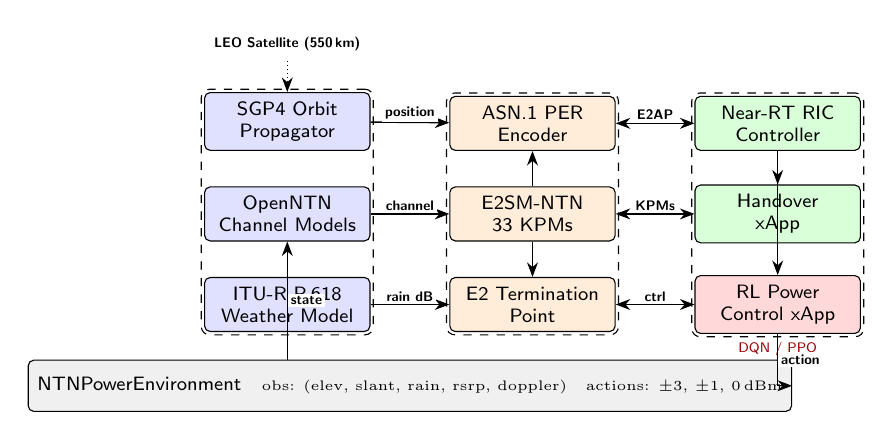
\begin{tikzpicture}[
    >=Stealth,
    node distance=0.45cm and 0.35cm,
    font=\sffamily\scriptsize,
    box/.style={draw, rounded corners=2pt, minimum height=0.65cm,
                minimum width=2.1cm, align=center, line width=0.4pt},
    bigbox/.style={draw, rounded corners=3pt, dashed, line width=0.4pt,
                   inner sep=5pt, fill opacity=0.08},
    arrow/.style={->, thick, line width=0.5pt},
    darrow/.style={<->, thick, line width=0.5pt},
    label/.style={font=\sffamily\tiny\bfseries, fill=white, inner sep=1pt},
]

% === Left column: Physical Layer ===
\node[box, fill=blue!12] (sgp4) {SGP4 Orbit\\Propagator};
\node[box, fill=blue!12, below=of sgp4] (openntn) {OpenNTN\\Channel Models};
\node[box, fill=blue!12, below=of openntn] (weather) {ITU-R P.618\\Weather Model};

% Group: Physical layer
\begin{scope}[on background layer]
  \node[bigbox, fill=blue!5, fit=(sgp4)(openntn)(weather),
        label={[label, anchor=south]above:Physical Layer}] (phys) {};
\end{scope}

% === Middle column: E2 Interface ===
\node[box, fill=orange!15, right=1.0cm of openntn] (e2sm) {E2SM-NTN\\33 KPMs};
\node[box, fill=orange!15, above=of e2sm] (asn1) {ASN.1 PER\\Encoder};
\node[box, fill=orange!15, below=of e2sm] (e2term) {E2 Termination\\Point};

% Group: E2 Interface
\begin{scope}[on background layer]
  \node[bigbox, fill=orange!5, fit=(e2sm)(asn1)(e2term),
        label={[label, anchor=south]above:E2 Interface}] (e2grp) {};
\end{scope}

% === Right column: Near-RT RIC ===
\node[box, fill=green!15, right=1.0cm of asn1] (ric) {Near-RT RIC\\Controller};
\node[box, fill=green!15, right=1.0cm of e2sm] (hoapp) {Handover\\xApp};
\node[box, fill=red!15, right=1.0cm of e2term] (pwapp) {RL Power\\Control xApp};

% RL sub-labels
\node[font=\sffamily\tiny, below=-0.02cm of pwapp, text=red!60!black]
     {DQN / PPO};

% Group: Near-RT RIC
\begin{scope}[on background layer]
  \node[bigbox, fill=green!5, fit=(ric)(hoapp)(pwapp),
        label={[label, anchor=south]above:Near-RT RIC}] (ricgrp) {};
\end{scope}

% === Bottom: NTN Environment ===
\node[box, fill=gray!12, minimum width=6.8cm,
      below=0.7cm of $(e2term)!0.5!(weather)$] (env)
     {NTNPowerEnvironment\quad
      \normalfont\tiny obs: (elev, slant, rain, rsrp, doppler)\quad
      actions: $\pm$3, $\pm$1, 0\,dBm};

% === Arrows: Physical layer -> E2 ===
\draw[arrow] (sgp4)   -- node[label, above, pos=0.5] {position} (asn1);
\draw[arrow] (openntn) -- node[label, above, pos=0.5] {channel} (e2sm);
\draw[arrow] (weather) -- node[label, above, pos=0.5] {rain dB}  (e2term);

% === Arrows: E2 internal ===
\draw[arrow] (e2sm) -- (asn1);
\draw[arrow] (e2sm) -- (e2term);

% === Arrows: E2 <-> RIC ===
\draw[darrow] (asn1)   -- node[label, above, pos=0.5] {E2AP} (ric);
\draw[darrow] (e2sm)   -- node[label, above, pos=0.5] {KPMs}  (hoapp);
\draw[darrow] (e2term) -- node[label, above, pos=0.5] {ctrl}   (pwapp);

% === Arrows: RIC internal ===
\draw[arrow] (ric) -- (hoapp);
\draw[arrow] (ric) -- (pwapp);

% === Arrows: Environment ===
\draw[arrow] (env.north -| openntn) -- (openntn.south)
     node[label, right, pos=0.5] {state};
\draw[arrow] (pwapp.south) |- (env.east)
     node[label, right, pos=0.25] {action};

% === LEO satellite icon (top) ===
\node[above=0.4cm of sgp4, font=\sffamily\tiny\bfseries] (sat)
     {LEO Satellite (550\,km)};
\draw[arrow, densely dotted] (sat) -- (sgp4);

\end{tikzpicture}
\end{document}
